% Author: Dr. Matthias Jung, DL9MJ
% Year: 2021
\documentclass[convert = false, border=5pt]{standalone}
\usepackage{fontspec}
\setmainfont{Roboto}
\usepackage[siunitx, straightvoltages, europeanresistors, european inductor]{circuitikzgit}
\usepackage{tikz}


\usetikzlibrary{calc, positioning}
\usepackage[siunitx, straightvoltages]{circuitikzgit}
\usepackage{pgfplotstable}
\usepackage{amsmath}
\usepackage{unicode-math}
\setmathfont{Fira Math}
\setmathfont[range=up]{Roboto}
\setmathfont[range=it]{Roboto-Italic}
\setmathfont[range=\int]{Fira Math}
\usepackage[euler]{textgreek}
\usetikzlibrary{calc, positioning}
\usepackage{pgfplots}
\usetikzlibrary{pgfplots.polar}
\pgfplotsset{width=16cm,compat=1.10}
\usepackage{MnSymbol}

\newcommand\TikCircle[1][2.5]{\tikz[baseline=-#1]{\draw[thick](0,0)circle[radius=#1mm];}}

\pgfplotsset{
    standard/.style={
        axis x line=middle,
        axis y line=left,
        ticklabel style={fill=white},
        set layers=tick labels on top% use layers and choose the new layer set
    },
    layers/tick labels on top/.define layer set=% define the new layer set based on the standard one
        {axis background,axis grid,axis ticks,axis lines,main,%
          axis tick labels,% <- tick labels before main
          axis descriptions,axis foreground}
        {/pgfplots/layers/standard}
}

\begin{document}
    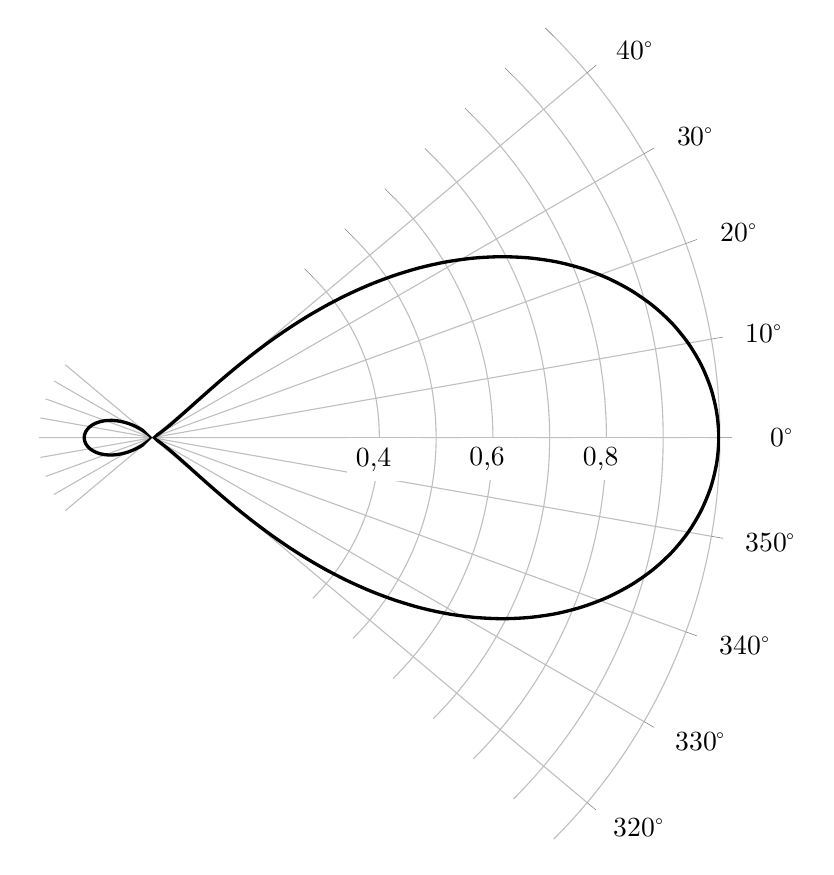
\begin{tikzpicture}[remember picture]


        \begin{polaraxis}[
            /pgf/number format/.cd,
            use comma,
            domain=-180:180,
            ymin=-0.2,
            ymax=1.0,
            xmin=-45,
            xmax=45,
            axis line style={draw=none},
            ytick={0.4,0.5,0.6,0.7,0.8,0.9,1.0},
            xtick={-40,-30,-20,-10,0,10,20,30,40},
            xticklabel={$\pgfmathprintnumber{\tick}^{\circ}$},
            xticklabel style={
                xshift=8.0
            },
            yticklabel={$\pgfmathprintnumber{\tick}$},
            yticklabel style={
              rotate=-45, 
              rotate around={45:(current axis.origin)},
              xshift=-12.0, 
              below right, 
              alias=ytick-\ticknum,
              fill=white,
            },
            y tick label style={
              /pgf/number format/.cd,
              fixed,
              fixed zerofill,
              precision=1,
              /tikz/.cd,
              fill=white,
            },
            yticklabels={0{,}4,~,0{,}6,~,0{,}8,~,~},
            xticklabels={$320^{\circ}$,$330^{\circ}$,$340^{\circ}$,$350^{\circ}$,$~~0^{\circ}$,$10^{\circ}$,$20^{\circ}$,$30^{\circ}$,$40^{\circ}$},
        ]
            %\addplot {1};

    \draw[very thick] plot[
          variable=\t,
          domain=0:360,
          smooth,samples=101
      ] 
    ({40*sin(\t)}:{129*pow(0.95*sin(\t/2),5)});

        \draw[very thick] plot[
        variable=\t,
        domain=0:360,
        smooth,samples=101
    ] 
    ({180+40*sin(\t)}:{12*pow(sin(\t/2),9)});

        \draw (-139.6,3.6) node[](origin){};

        \end{polaraxis}
    \end{tikzpicture}

\begin{tikzpicture}[overlay, remember picture, scale=1]
    \draw[very thick] (origin.south) -- ++(0,-0.8);
    \draw[very thick] (origin.south) -- ++(0, 0.8);

    \draw[very thick] (origin.south) ++(0.3,0) -- ++(0.0,-0.7);
    \draw[very thick] (origin.south) ++(0.3,0) -- ++(0.0, 0.7);

    \draw[very thick] (origin.south) ++(0.6,0) -- ++(0.0,-0.6);
    \draw[very thick] (origin.south) ++(0.6,0) -- ++(0.0, 0.6);

    \draw[very thick] (origin.south) ++(0.9,0) -- ++(0.0,-0.5);
    \draw[very thick] (origin.south) ++(0.9,0) -- ++(0.0, 0.5);

    \draw[very thick] (origin.south) ++(1.2,0) -- ++(0.0,-0.4);
    \draw[very thick] (origin.south) ++(1.2,0) -- ++(0.0, 0.4);

    \draw[very thick] (origin.south) ++(1.5,0) -- ++(0.0,-0.3);
    \draw[very thick] (origin.south) ++(1.5,0) -- ++(0.0, 0.3);

    \draw[thick, -Triangle] (origin.south) ++(0,0) -- ++(7.7, 0.0);
    \draw[thick] (origin.south) ++(0,0) -- ++(-1.45, 0.0);

    \draw[](origin.south) ++(3.60, 0.255) node [fill=white,rounded corners=2pt,inner sep=1pt](){d};
    \draw[](origin.south) ++(5.05, 0.220) node [fill=white,rounded corners=2pt,inner sep=1pt](){c};
    \draw[](origin.south) ++(6.10, 0.255) node [fill=white,rounded corners=2pt,inner sep=1pt](){b};
    \draw[](origin.south) ++(7.15, 0.225) node [fill=white,rounded corners=2pt,inner sep=1pt](){a};
    \draw[](origin.south) ++(7.15,-0.225) node [fill=white,rounded corners=2pt,inner sep=1pt](){1};

    \draw[](origin.south) ++(7.6,-0.6) node [](){\small$\dfrac{\mathrm{E}}{\mathrm{E}_\mathrm{max}}$};

\end{tikzpicture}

\end{document}
